In this final section, we are gonna take a look at whether we can indicate not the main index itself, but rather its turning points. There are several different definitions of economic turning points, and no single standard exists for Germany. We apply the Bry–Boschan algorithm \citep{boschan1971programmed}, as implemented in the R package BCDating \citep{BCDating}, to identify the troughs and peaks of the main index, which serve as the groundtruth. The algorithm analyzes the data retrospectively and identifies turning points based on several criteria, such as minimum cycle or phase lengths. A trough corresponds to an expansion turning point, indicating that the economy is about to enter a growth phase, commonly referred to as a boom. Conversely, a peak signals the end of the previous expansion and the beginning of a contraction, typically known as a recession.
\begin{figure}[H]
\centering
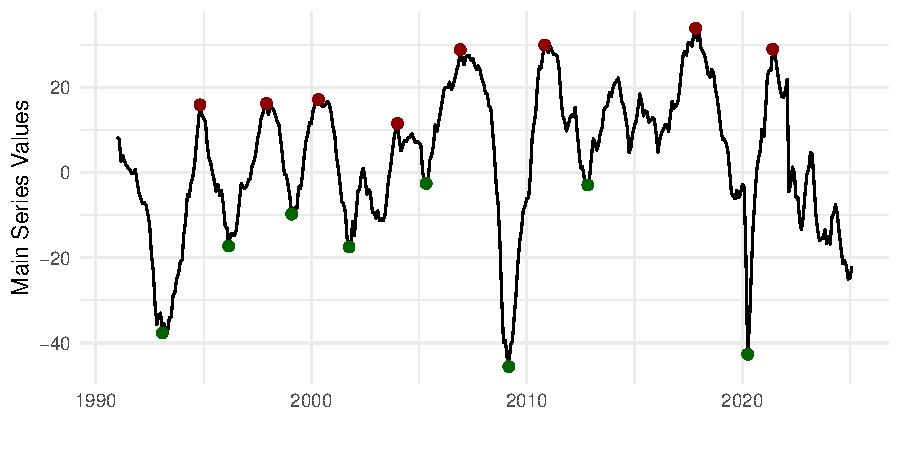
\includegraphics[width=0.5\linewidth]{JakobPlots/BB_main.pdf}
\caption{Bry-Boschan Turning Points of the main index.}
\end{figure}

\subsection{Markov-Regime-Switching}
To simulate a realistic real-time setting for potentially identifying subseries, the Bry-Boschan algorithm is not suitable, as it requires the full data range. Instead, we apply a two-regime Markov-switching model \citep{hamilton1989new}, which allows the system to switch between two regimes, $s_t$, each month and follow the implementation of the R package MSwM \citep{MSwM} for the model. The probability of switching is governed by a latent Markov chain, and each regime is characterized by a different intercept:
\[
y_t = \mu_{s_t} + \epsilon_t , \quad \epsilon_t \sim \mathcal{N}(0,\sigma^2),
\]

Each month, the model provides the probability of switching to the upper regime with a higher intercept in the following month. Following \citet{sauer2023handbook}, we apply a decision rule to classify turning points: if the probability of the upper regime exceeds 0.66 for the first time, it is considered an expansion turning point and if it falls below 0.33 for the first time, it indicates a contraction turning point. Probabilities between 0.33 and 0.66 are treated as uncertain and do not form a strong enough signal for a turning point yet.
\\
The above model can either be run with smoothed probabilities, meaning that the whole data range is used to fit the model, or filtered probabilities, where only data up to the current month $t$ is used. The later one simulates a real-time forecasting scenario and is thus suitable for our evaluation. Note that we did not perform any train-test split to evaluate forecasting models, this is rather a descriptive setting based on the past 30 years. 

\subsection{Classification Task}
Fitting the above to all individual level 1 series gives us turning points for all of these series. To evaluate whether these individual turning points, predicted in real-time, can indicate the groundtruth turning points of the main index, we see it as a classification task. A hit occurs if an actual main turning point follows within a fixed time window after a predicted one. Table~\ref{tab:tp_classification} shows the typical classification metrics we used. However, it also shows how no individual series did bring up any meaningful results, even when tolerating a three months delay for the predicted turning points, compared to the actual ones. 
\begin{table}[H]
\footnotesize
\centering
\begin{subtable}{\linewidth}
    \centering
    \makebox[\textwidth]{%
    \begin{tabular}{lllllllll}
    \toprule
    \textbf{Industry} & \textbf{Question} & \textbf{Hits} & \textbf{Total Pred} & \textbf{Total Actual} & \textbf{Precision} & \textbf{Recall} & \textbf{F1} & \textbf{Lead Time (sd)} \\
    \midrule
    C1900000 & PVS & 7 & 47 & 16 & 0.151 & 0.438 & 0.224 & 2.96 (2.76) \\
    C2000000 & LUS & 4 & 20 & 16 & 0.202 & 0.250 & 0.223 & 5.00 (1.41) \\
    C1300000 & PWS & 4 & 20 & 16 & 0.200 & 0.250 & 0.222 & 4.00 (2.00) \\
    \bottomrule
    \end{tabular}%
    }
    \caption{0 - 6 Months Lead time}
    \label{tab:tp_classification}
\end{subtable}

\vspace{0.5em}
\begin{subtable}{\linewidth}
    \centering
    \makebox[\textwidth]{%
    \begin{tabular}{lllllllll}
    \toprule
    \textbf{Industry} & \textbf{Question} & \textbf{Hits} & \textbf{Total Pred} & \textbf{Total Actual} & \textbf{Precision} & \textbf{Recall} & \textbf{F1} & \textbf{Lead Time (sd)} \\
    \midrule
    C2000000 & QES & 5 & 21 & 16 & 0.312 & 0.312 & 0.312 & -0.60 (2.88) \\
    C1900000 & PVS & 9 & 47 & 16 & 0.196 & 0.562 & 0.291 & 2.17 (3.05) \\
    C1900000 & PWS & 6 & 27 & 16 & 0.225 & 0.375 & 0.280 & 2.00 (3.34) \\
    \bottomrule
    \end{tabular}%
    }
    \caption{-3 - 6 Months Lead time}
\end{subtable}
\end{table}
Since individual series did not appear to provide meaningful signals, we explored grouping multiple series to see if a combined signal could yield a reliable indication. We tested several approaches for aggregating turning points across series: collecting turning points within a rolling window and signaling if a certain threshold was exceeded; averaging their binary states based on the most recent turning point; and averaging the Markov-switching probabilities across series, followed by applying the 0.33/0.66 decision rule. \\
We also used several different approaches to form the groups, such as simply aligning series by their lag value with peak correlation or switching to level 2 and using the groups obtained from CCF-based clustering. However, none of these approaches produced meaningful or interpretable signals.
\subsubsection{Grouped Series - Flipped}
However, a small effect was observed when noting that, for some groups, the approximate number of turning points roughly matched the number of ground-truth turning points. For instance, considering all series with peak CCFs at lags -1, 0, and 1, so series with roughly synchronous characteristics. Their turning points were lagging quite far behind the Bry-Boschan turning points of the main index, potentially also simply due to the nature of using a Markov switching model with differing intercepts. But flipping the prediction goal and predicting opposite turning points, predicting contraction points as expansions and vice versa, the subseries do seem to roughly indicate main turning points. Whether this has any actual value is open, but a potential interpretation might be that once even these groups have reached the current regime according to their Markov switching probability, it might soon be over and a turning point could occur in the next twelve months. Fig.~\ref{fig:flipped_turningpoints} shows the turning points of the above group compared to the main ones and table~\ref{tab:flipped_turningpoints} the scores when evaluating according to this flipped scenario. 

\begin{figure}[H]
    \centering
    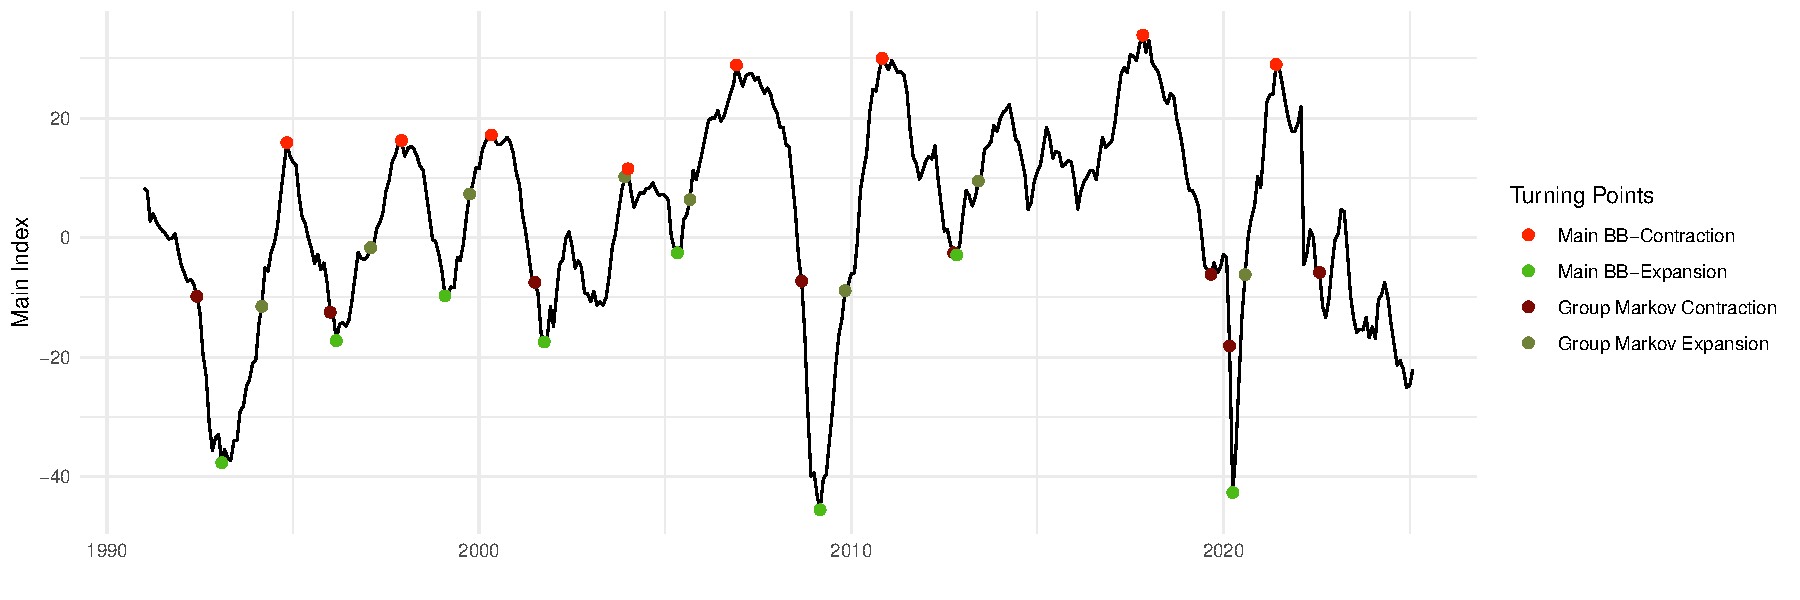
\includegraphics[width=\linewidth]{JakobPlots/Lag1_3_cluster_turningpoints_main.pdf}
    \caption{Turning points of group of all level 1 series with roughly composite moving characteristics according to their peak CCF lag value.}
    \label{fig:flipped_turningpoints}
\end{figure}

\begin{table}[H]
\centering
\footnotesize
\makebox[\textwidth]{%
\begin{tabular}{lllllllll}
\toprule
\textbf{Main Type} & \textbf{Hits} & \textbf{Total Pred} & \textbf{Total Actual} & \textbf{Precision} & \textbf{Recall} & \textbf{F1} & \textbf{Lead Time (sd)}\\
\midrule
Expansion & 6 & 7 & 8 & 0.857 & 0.75 & 0.8 & 5.67 (3.78) \\
Contraction & 6 & 8 & 8 & 0.75 & 0.75 & 0.75 & 3.17 (3.37) \\
\bottomrule
\end{tabular}
}
\caption{Evaluation of the flipped indication setting.}
\label{tab:flipped_turningpoints}
\end{table}
